\documentclass[sigconf]{acmart}
\usepackage{tikz}
\usetikzlibrary{shapes.geometric}
\usetikzlibrary{matrix}
\usetikzlibrary{graphs}
\usetikzlibrary{shapes.geometric}
\usepackage{pgfplots}
\pgfplotsset{compat=1.18} % Recommended for modern TikZ/pgfplots
\usepackage{environ}
\usepackage{ifthen}
\usepackage{graphicx}
\usepackage{subcaption}
\usepackage{fp}
\usepackage{makecell}
%%
%% \BibTeX command to typeset BibTeX logo in the docs
\AtBeginDocument{%
  \providecommand\BibTeX{{%
    Bib\TeX}}}

\setcopyright{acmlicensed}
\copyrightyear{2026}
\acmYear{2026}
\setcopyright{cc}
\setcctype{by}
\acmConference[FPGA '26]{Proceedings of the 2026 ACM/SIGDA International Symposium on Field Programmable Gate Arrays}{February 22--24, 2026}{Seaside, CA, USA}
\acmBooktitle{Proceedings of the 2026 ACM/SIGDA International Symposium on Field Programmable Gate Arrays (FPGA '26), February 22--24, 2026, Seaside, CA, USA}
\acmPrice{}
\acmDOI{10.1145/3748173.3779548}
\acmISBN{979-8-4007-2079-6/2026/02}

%%
%%  Uncomment \acmBooktitle if the title of the proceedings is different
%%  from ``Proceedings of ...''!
%%
%%\acmBooktitle{Woodstock '18: ACM Symposium on Neural Gaze Detection,
%%  June 03--05, 2018, Woodstock, NY}

\begin{document}

\title{Multi-Port Memory with Bidirectional Ports for FPGAs Using XOR and LVT Methods}

%%
%% The "author" command and its associated commands are used to define
%% the authors and their affiliations.
%% Of note is the shared affiliation of the first two authors, and the
%% "authornote" and "authornotemark" commands
%% used to denote shared contribution to the research.
\author{Kevin Townsend}
\orcid{0000-0003-2022-7133}
\affiliation{%
  \institution{Unaffiliated}
  \city{Sunnyvale}
  \state{CA}
  \country{USA}}
\email{kevintownsend4219@gmail.com}

\renewcommand{\shortauthors}{Townsend}

\begin{abstract}
  We propose a generalization to a previous XOR memory implementation to allow for any number of full, read-only, and write-only ports.
This implementation creates these additional ports by encoding and decoding the data entries with XOR logic. The incoming (written) data is encoded with the data corresponding to the other ports and the outgoing (read) data is decoded by XORing all the entries in the memory banks.
Using XOR operators to accomplish this encoding/decoding has advantages over other approaches because the XOR operator is a simple and efficient operation.
The result is a high-throughput multi-ported memory that is particularly well-suited for implementation on FPGAs.
We also implemented an efficient architecture for creating a live value table (LVT) memory using an XOR-based scheme by utilizing its bidirectional capabilities.
We use an XOR memory with full ports to implement a bidirectional live value table design.
We evaluate the architecture's performance and resource utilization, and show that the XOR-based bidirectional live value table is a compelling alternative for applications requiring high-performance, flexible memory access.
\end{abstract}

%%
%% The code below is generated by the tool at http://dl.acm.org/ccs.cfm.
%% Please copy and paste the code instead of the example below.
%%
%\begin{CCSXML}
%<ccs2012>
% <concept>
%  <concept_id>00000000.0000000.0000000</concept_id>
%  <concept_desc>Do Not Use This Code, Generate the Correct Terms for Your Paper</concept_desc>
%  <concept_significance>500</concept_significance>
% </concept>
% <concept>
%  <concept_id>00000000.00000000.00000000</concept_id>
%  <concept_desc>Do Not Use This Code, Generate the Correct Terms for Your Paper</concept_desc>
%  <concept_significance>300</concept_significance>
% </concept>
% <concept>
%  <concept_id>00000000.00000000.00000000</concept_id>
%  <concept_desc>Do Not Use This Code, Generate the Correct Terms for Your Paper</concept_desc>
%  <concept_significance>100</concept_significance>
% </concept>
% <concept>
%  <concept_id>00000000.00000000.00000000</concept_id>
%  <concept_desc>Do Not Use This Code, Generate the Correct Terms for Your Paper</concept_desc>
%  <concept_significance>100</concept_significance>
% </concept>
%</ccs2012>
%\end{CCSXML}
%
%\ccsdesc[500]{Do Not Use This Code~Generate the Correct Terms for Your Paper}
%\ccsdesc[300]{Do Not Use This Code~Generate the Correct Terms for Your Paper}
%\ccsdesc{Do Not Use This Code~Generate the Correct Terms for Your Paper}
%\ccsdesc[100]{Do Not Use This Code~Generate the Correct Terms for Your Paper}

%%
%% Keywords. The author(s) should pick words that accurately describe
%% the work being presented. Separate the keywords with commas.
%\keywords{Do, Not, Us, This, Code, Put, the, Correct, Terms, for,
%  Your, Paper}
%% A "teaser" image appears between the author and affiliation
%% information and the body of the document, and typically spans the
%% page.
\begin{teaserfigure}
  %\includegraphics[width=\textwidth]{sampleteaser}
  \centering
  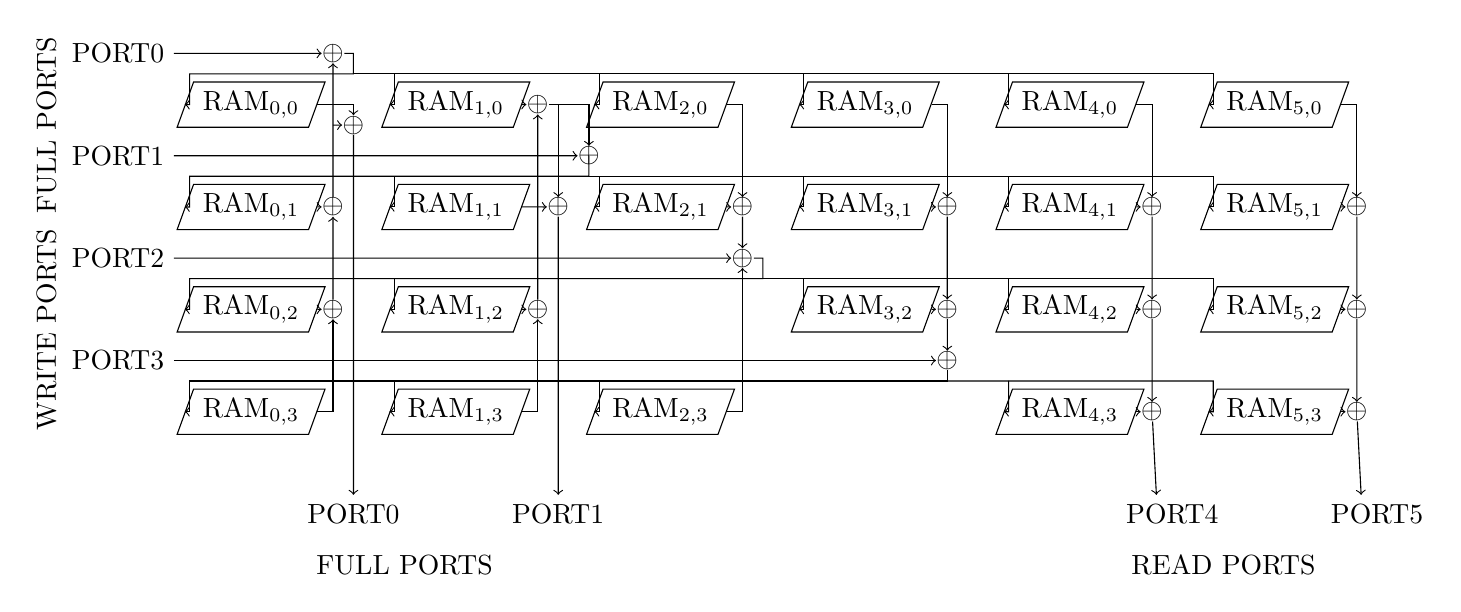
\begin{tikzpicture}[scale=1.3]
  \foreach \x in {0,1,2,3,4,5} {
    \foreach \y in {0,1,2,3} {
      \ifthenelse{\(\x = 2 \AND \y = 1\) \OR \(\x = 3 \AND \y = 0\)}{}{
        \node (r\x\y)[trapezium, trapezium left angle=70, trapezium right angle=110, draw] at (2*\x, \y){RAM$_{\x,\fpeval{3-\y}}$};
      }
    }
  }
  \foreach \x in {0,1,4,5} {
    \node (bport\x)[] at (2*\x+1, -1){PORT\x};
  }
  \foreach \y in {0,1,2,3} {
    \node (lport\y)[] at (-1.3, 3.5-\y){PORT\y};
  }
  \node [rotate=90] at (-2, .8){WRITE PORTS};
  \node [rotate=90] at (-2, 2.8){FULL PORTS};
  \node [] at (1.5, -1.5){FULL PORTS};
  \node [] at (9.5, -1.5){READ PORTS};
  \node(x50)[inner sep=0pt] at (10.8, 0){$\oplus$};
  \node(x51)[inner sep=0pt] at (10.8, 1){$\oplus$};
  \node(x52)[inner sep=0pt] at (10.8, 2){$\oplus$};
  \draw[->] (r50) -- (x50);
  \draw[->] (r51) -- (x51);
  \draw[->] (r52) -- (x52);
  \draw[->] (r53) -| (x52);
  \draw[->] (x52) -- (x51);
  \draw[->] (x51) -- (x50);
  \draw[->] (x50) -- (bport5.130);
  \node(x40)[inner sep=0pt] at (8.8, 0){$\oplus$};
  \node(x41)[inner sep=0pt] at (8.8, 1){$\oplus$};
  \node(x42)[inner sep=0pt] at (8.8, 2){$\oplus$};
  \draw[->] (r40) -- (x40);
  \draw[->] (r41) -- (x41);
  \draw[->] (r42) -- (x42);
  \draw[->] (r43) -| (x42);
  \draw[->] (x42) -- (x41);
  \draw[->] (x41) -- (x40);
  \draw[->] (x40) -- (bport4.130);
  \node(x31)[inner sep=0pt] at (6.8, 1){$\oplus$};
  \node(x32)[inner sep=0pt] at (6.8, 2){$\oplus$};
  \node(x30)[inner sep=0pt] at (6.8, .5){$\oplus$};
  \draw[->] (r31) -- (x31);
  \draw[->] (r32) -- (x32);
  \draw[->] (r33) -| (x32);
  \draw[->] (x32) -- (x31);
  \draw[->] (x31) -- (x30);
  %PORT3 connections.
  \draw[->] (lport3) -- (x30);
  \draw[->] (x30) |- (-.6,.3) |- (r00);
  \draw[->] (1.4,.3) |- (r10);
  \draw[->] (3.4,.3) |- (r20);
  \draw[->] (6.8, .3) -| (7.4,0) -- (r40);
  \draw[->] (7.4, .3) -| (9.4,0) -- (r50);
  %PORT2 XORs
  \node(x22)[inner sep=0pt] at (4.8, 2){$\oplus$};
  \node(x21)[inner sep=0pt] at (4.8, 1.5){$\oplus$};
  %PORT2 connections
  \draw[->] (lport2) -- (x21);
  \draw[->] (r23) -| (x22);
  \draw[->] (r22) -- (x22);
  \draw[->] (x22) -- (x21);
  \draw[->] (r20) -| (x21);
  \draw[->] (x21) -| (5,1.3) -| (-.6,1) -- (r01);
  \draw[->] (1.4,1.3) |- (r11);
  \draw[->] (5,1.3) -- (9.4, 1.3) |- (r51);
  \draw[->] (7.4, 1.3) |- (r41);
  \draw[->] (5.4, 1.3) |- (r31);
  %draw xor of full ports
  %PORT1
  \node(x11)[inner sep=0pt] at (2.8, 1){$\oplus$};
  \node(x12)[inner sep=0pt] at (3.3, 2.5){$\oplus$};
  \node(x12b)[inner sep=0pt] at (3, 2){$\oplus$};
  \node(x13)[inner sep=0pt] at (2.8, 3){$\oplus$};
  \draw[->] (r10) -| (x11);
  \draw[->] (r11) -- (x11);
  \draw[->] (lport1) -- (x12);
  \draw[->] (x11) -- (x13);
  \draw[->] (r13) -- (x13);
  \draw[->] (x13) -| (x12);
  \draw[->] (r12) -- (x12b);
  \draw[->] (x12) -| (3.3, 2.3) -| (-.6,2) -- (r02);
  \draw[->] (1.4,2.3) |- (r12);
  \draw[->] (3.3, 2.3) -- (9.4, 2.3) |- (r52);
  \draw[->] (3.4, 2.3) |- (r22);
  \draw[->] (5.4, 2.3) |- (r32);
  \draw[->] (7.4, 2.3) |- (r42);
  \draw[->] (x13) -| (x12b);
  \draw[->] (x12b) -- (bport1);
  %PORT0
  \node(x01)[inner sep=0pt] at (0.8, 1){$\oplus$};
  \node(x02)[inner sep=0pt] at (0.8, 2){$\oplus$};
  \node(x03)[inner sep=0pt] at (0.8, 3.5){$\oplus$};
  \node(x03b)[inner sep=0pt] at (1.0, 2.8){$\oplus$};
  \draw[->] (r00) -| (x01);
  \draw[->] (r01) -- (x01);
  \draw[->] (x01) -- (x02);
  \draw[->] (x02) -- (x03);
  \draw[->] (lport0) -- (x03);
  \draw[->] (x03) -| (1, 3.3) -| (-.6,3) -- (r03);
  \draw[->] (1, 3.3) -- (9.4, 3.3) |- (r53);
  \draw[->] (1.4, 3.3) |- (r13);
  \draw[->] (3.4, 3.3) |- (r23);
  \draw[->] (5.4, 3.3) |- (r33);
  \draw[->] (7.4, 3.3) |- (r43);
  \draw[->] (.8, 2.8) -- (x03b);
  \draw[->] (r02) -- (x02);
  \draw[->] (r03) -| (x03b);
  \draw[->] (x03b) -- (bport0);
  \end{tikzpicture}
  %\end{scaletikzpicturetowidth}
  %\end{center}
  \caption{A multi-port memory with 2 full ports, 2 write-only ports and 2 read-only ports.}
  \Description{Enjoying the baseball game from the third-base
  seats. Ichiro Suzuki preparing to bat.}
  \label{fig:teaser}
\end{teaserfigure}

%\received{1 Octomber 2025}
%\received[revised]{XX XXX XXXX}
%\received[accepted]{XX XXX XXXX}

%%
%% This command processes the author and affiliation and title
%% information and builds the first part of the formatted document.
\maketitle

\section{Source Code}
We provide all of the source code used in implementation and testing our design at
https://github.com/kevintownsend/mpm. We tested our design with Verilator\cite{verilator_manual} and synthesized the design
with Vivado\cite{ug893} targeting an AMD Virtex UltraScale+ HBM VU47P-3 FPGA.

\section{Generalizing XOR memory}

We propose a simple generalization to XOR memories presented in previous work\cite{laforest14}.
Figure \ref{fig:teaser} demonstrates how to create an XOR memory with 2 read ports, 2 write ports and 2 full ports, which requires 22 RAMs.

%% The next two lines define the bibliography style to be used, and
%% the bibliography file.
\bibliographystyle{ACM-Reference-Format}
\bibliography{paper}


%%
%% If your work has an appendix, this is the place to put it.
%\appendix

\end{document}
\endinput
%%
%% End of file `sample-sigconf.tex'.
